
\documentclass{article}

\usepackage{fullpage}
\usepackage{graphicx}
\usepackage{amsmath}
\usepackage{textcomp}

\title{Incompressible Navier Stokes Simulation}
\author{Michael Deakin}

\begin{document}
\maketitle

\begin{section}{Introduction}
In this report, I describe the properties of the Implicit Euler solver written for the incompressible Navier-Stokes equations with an artificial compressibility method.
This solver was implemented with a second order centered finite volume spatial discretization,
with Neumann boundary conditions on the pressure equation and Dirichlet conditions on the velocity components.
The pressure equation was slightly modified with the addition of a diffusion term to reduce the ringing in the solution,
and over-relaxation was also implemented to reduce the time to solution.
A parameter study was employed to estimate reasonable choices for the compressibility parameter,
the amount to over-relax, and the amount of diffusion to add.
Several tests were employed to ensure the solution was reasonable,
and that it exhibited second order convergence.

To run this code, I exported a Python interface with Pybind11.
Because it's not trivial, a script to install Pybind11 on Ubuntu can be found in the
.travis.yml file in the root directory.
The scripts used to generate the figures in this report are in the ``scripts'' directory,
they need to be run from the same directory as the ``ins\_solver'' Python module library;
CMake was configured to copy them to the build directory upon modification to simplify this.
Note that when running them you also need to make certain to use the same Python version
as the module was built for, which likely means changing the shell command at the start of the files.
\end{section}

\begin{section}{Spatial Discretization}
A second order centered finite volume scheme was used as the spatial discretization.
Two steps were taken to ensure that the necessary components were implemented correctly here:
\begin{itemize}
{\item
  A test of the flux integral, which verified it converged to a known solution with second order;
  the results of this are in Table \ref{flux_int}.
}
{\item
  A test of the Jacobian, which verified that using it to linearly approximate the change in the
  flux integral components gave a reasonable answer.
  This test was performed with a $\Delta P = \Delta u = \Delta v = 1E-6$;
  the errors of this approximation of the flux integral are shown in Table \ref{jacobian}.
}
\end{itemize}

\begin{table}[ht]
  \centering{
  \begin{tabular}{|c|c|c|c|c|}
    \hline
    Mesh      & Pressure    & Pressure    & U Velocity  & U Velocity \\
              & $L^2$ Error & Convergence & $L^2$ Error & Convergence\\
    \hline
    10 x 10   & 0.0479469   & --          & 0.685970    & --    \\
    20 x 20   & 0.0119834   & 2.000       & 0.173420    & 1.984 \\
    40 x 40   & 0.00299570  & 2.000       & 0.0434765   & 1.996 \\
    80 x 80   & 0.000748916 & 2.000       & 0.0108767   & 1.999 \\
    160 x 160 & 0.000187228 & 2.000       & 0.0027197   & 2.000 \\
    \hline
  \end{tabular}
  \label{flux_int}
  \caption{Test of the flux integral implementation.
    Because the $u$ and $v$ velocity components were symmetric, the $v$ component was omitted}
  }
\end{table}

\begin{table}[ht]
  \begin{tabular}{|c|c|c|c|}
    \hline
    Center Offset & Pressure Error & U Velocity Error & V Velocity Error\\
    \hline
    $(0, -1)$     & -8.88E-16      & -4.99E-12        & -5.01E-12       \\
    $(-1, 0)$     & -8.88E-16      & -4.99E-12        & -5.01E-12       \\
    $(0, 0)$      &  2.00E-15      & -4.97E-14        &  2.13E-14       \\
    $(1, 0)$      & -2.22E-16      &  5.01E-12        &  5.01E-12       \\
    $(0, 1)$      & -2.22E-16      &  5.01E-12        &  4.99E-12       \\
    \hline
  \end{tabular}
  \label{jacobian}
  \caption{The error in a linear approximation of the change in the
    flux integral's value based on the Jacobian.
    A 20x20 mesh was used, with all components varied by $1E-6$.}
\end{table}
\end{section}

Both of these tests were applied to the initial conditions in Figure \ref{initial_conds}.
\begin{figure}[ht]
  \hspace{-30mm}
  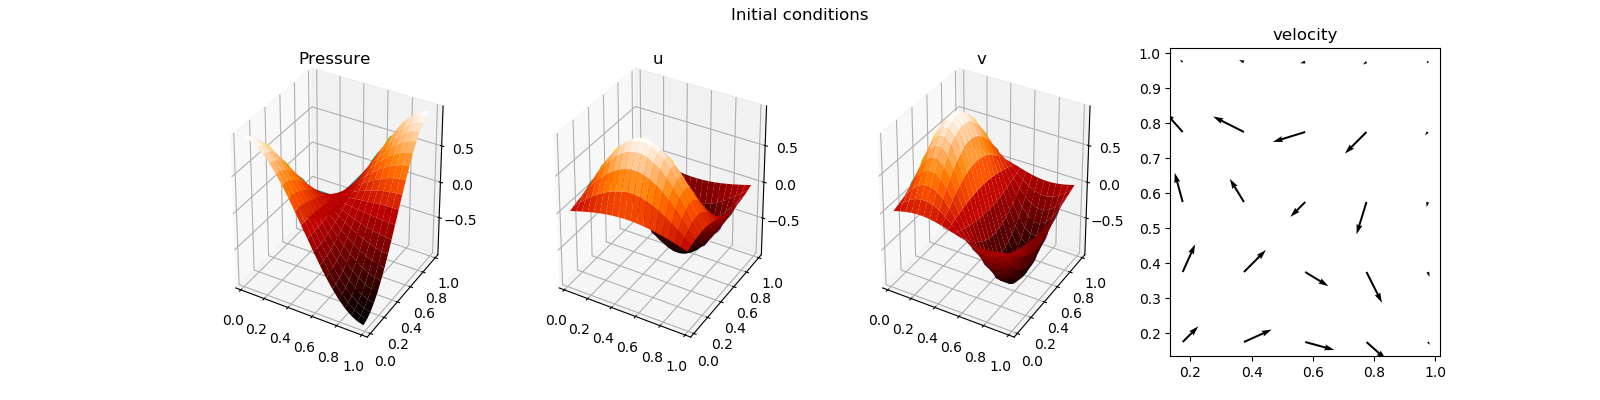
\includegraphics[width=1.35\textwidth]{initial_conds/initial_conds.png}
  \label{initial_conds}
  \caption{The initial conditions of the system}
\end{figure}

\begin{section}{Time Discretization}
An analytic solution for the time evolution of our system was not known (by me),
so instead we only test for stability and convergence.
Then by Lax's consistency theorem we know we've come to the solution of the equations
(assuming they were implemented correctly) in the system.

To begin with, I start with the trivial case with fixed walls,
which has a trivial steady state solution, ie zero, for all of the components, everywhere.
The changes in $P, u, v$ from each iteration are shown in Figure \ref{trivial}.

\begin{figure}[ht]
  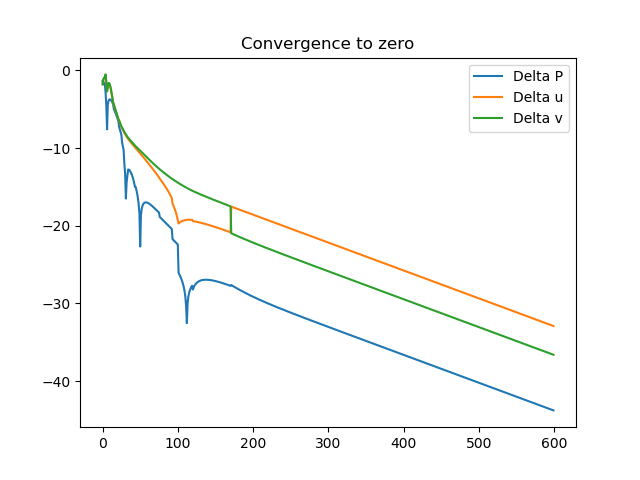
\includegraphics[width=0.45\textwidth]{trivial_sol/convergence.png}\\
  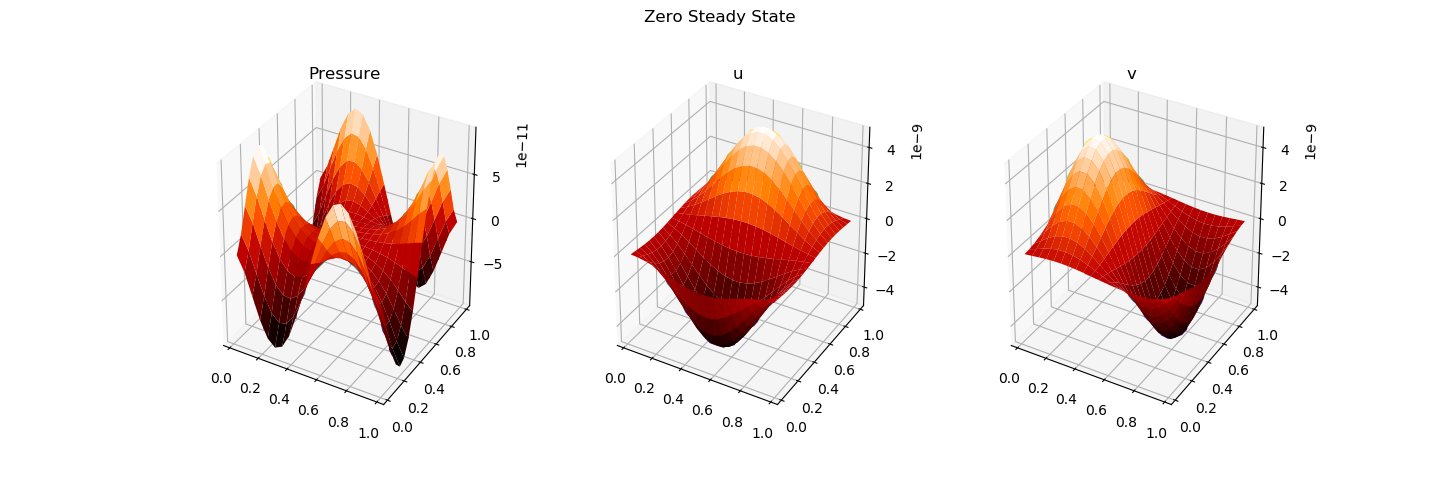
\includegraphics[width=0.95\textwidth]{trivial_sol/steadystate.png}
  \label{trivial}
  \caption{{\bf Top:} The change in $P, u, v$ vs iteration.
    {\bf Bottom:} The final steady state solution.
    This was run with a diffusion coefficient of 32.0 to reduce ringing.}
\end{figure}

The next case was nearly identical, except that the top wall was given a horizontal velocity of $1.0$.
This suffered from ringing in the corners with the inconsistent boundary conditions,
making the solution worse, but was important for verifying that it exhibited second order convergence with mesh size.
To test this, I ran the simulation with mesh sizes 10x10, 20x20, 40x40, 80x80, 160x160.
I assumed that the 160x160 mesh size was essentially the solution and used it to estimate the
order of convergence wrt mesh size.
The $L^2$ errors and the approximate rates of convergence at each mesh size are shown in Table \ref{mesh_convergence},
and a plot of the solution of $u$ down the middle is shown in Figure \ref{mesh_convergence_u_sym}.
The table shows that the order of convergence is increasing,
though larger meshes haven't been tried to show that the order of convergence stops at 2.0.
However, because we know the spatial discretization is at most 2.0,
we know it's not going to be larger than that, and it's unlikely to decrease,
so we conclude that it is indeed second order accurate.

\begin{table}[ht]
  \begin{tabular}{|c|c|c|c|}
    \hline
    Mesh Size & Pressure Convergence & U Velocity Convergence & V Velocity Convergence\\
    \hline
    20x20 & 0.965 & 1.19 & 1.14\\
    40x40 & 1.46 & 1.64 & 1.67\\
    80x80 & 1.92 & 2.15 & 2.12\\
    \hline
  \end{tabular}
  \label{mesh_convergence}
  \caption{Convergence of the error for $u=1.0$, a diffusion coefficient of 16.0,
    and over-relaxation of 1.5}
\end{table}

I also verified that negating the wall velocity and flipping the mesh about the $x=0.5$ line
produced the negative of the original $u$ velocity.
The result, not converged as far as I'd like (though it can be done), is shown in Figure \ref{u_sym}.

\begin{figure}[ht]
  \hspace{-30mm}
  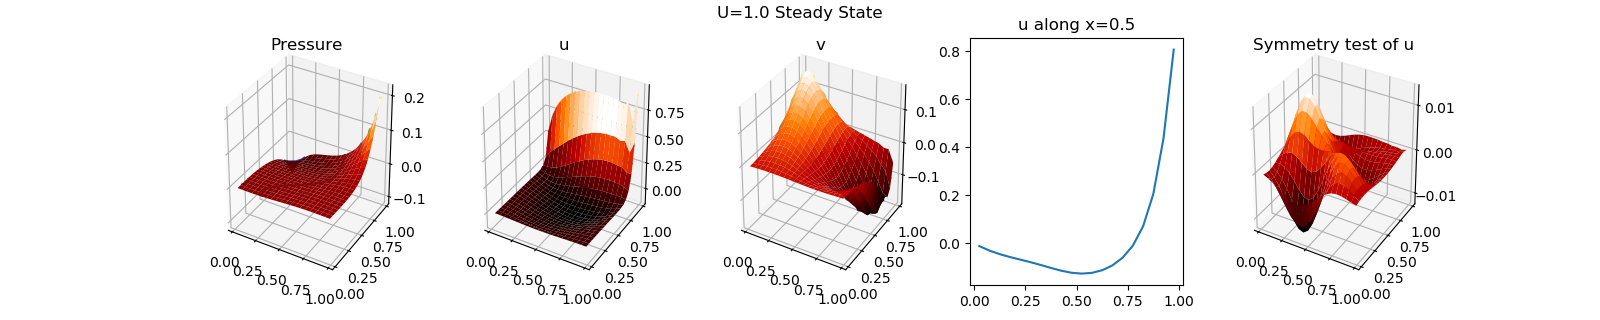
\includegraphics[width=1.35\textwidth]{mesh_convergence_u_sym/symmetry.png}
  \label{u_sym}
  \caption{{\bf From left to right:} The computed solutions of $P$, $u$, and $v$.
    The computed value of $u$ down the center of the mesh.
    The result the symmetry test on $u$.
  }
\end{figure}

\end{section}

\begin{section}{Solution Features}

After verifying the solver performed as expected, an analysis of the
features of the solution was performed.
In this case, it's expected that the solution will have a vortex near the top wall,
and possibly small eddies beneath it.
These features will likely be of the same scale as the domain,
with some amount of squashing in the vertical direction due to the difference in boundary conditions.
Indeed, such a result can be seen in Figure \ref{vortex_1}.
Not all features are visible in the original output, so some filtering is applied to better visualize the result.
Specifically, velocities below a threshold of 0.1 were increased by a factor of 10.0
to make their magnitudes comparable to the more distinct features.

\begin{figure}[ht]
  \hspace{-30mm}
  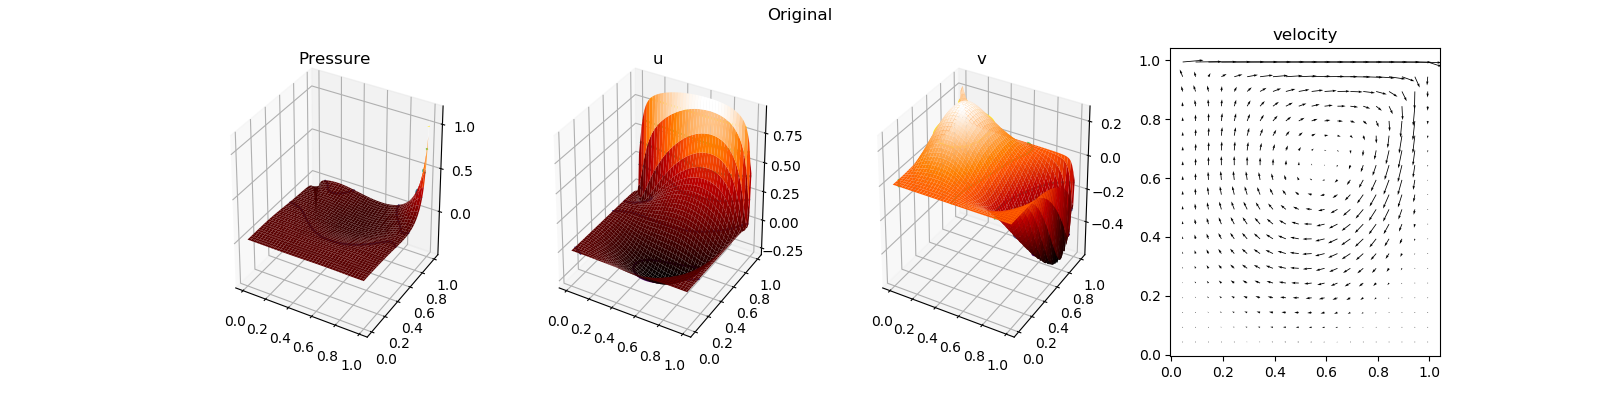
\includegraphics[width=1.35\textwidth]{vortices/original_single.png}

  \hspace{-30mm}
  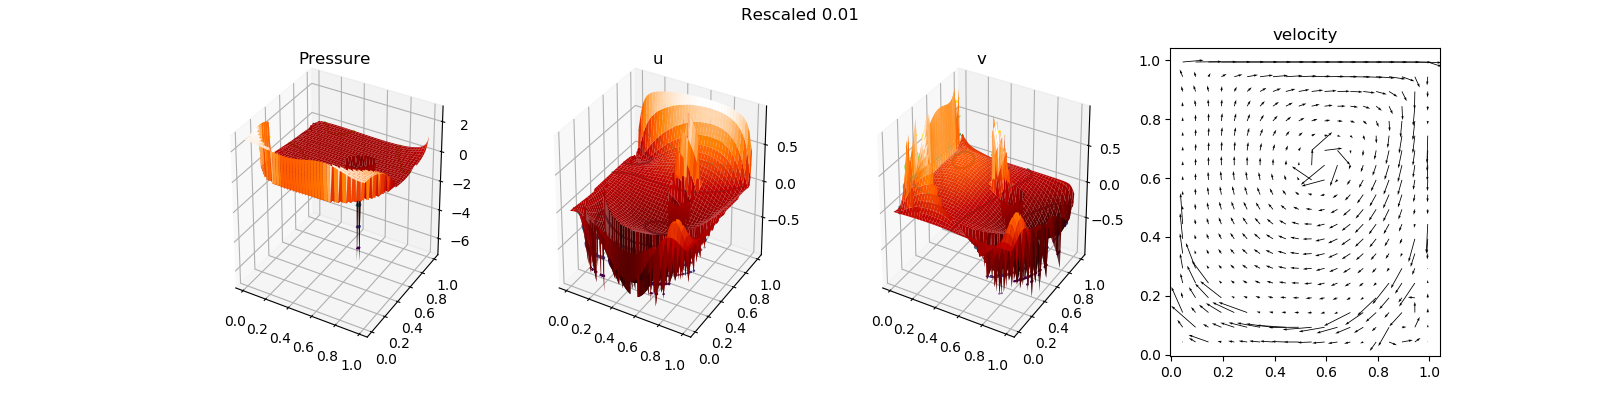
\includegraphics[width=1.35\textwidth]{vortices/rescaled_0_01_single.png}
  \label{vortex_1}
  \caption{{\bf From left to right, top to bottom:} The computed solutions of $P$, $u$, and $v$.
    The velocity of the solution. A filtered and rescaled version of the plot,
    showing a possible eddy in the lower right corner.
    This was run with an 80x80 mesh, over-relaxation of 1.25, beta of 0.75,
    and diffusion coefficient of 32.0}
  }
\end{figure}

Identifying the center of the vortex was done by a method which combines
the bisection and secant methods.
This method looks at a slice of the $u$ values at the line of $x$ symmetry in the mesh,
identifies $y$ values of the zeros, and then looks at a linearly interpolated slice of the $v$ values
at the determined $y$ values.
In principle, this method could be iterated further to better approximate the $x$ and $y$ values,
but due to the spatial discretization error being second order,
the accuracy will not be improved beyond a first pass.
From this I found the center of the vortex to be at about $(0.5873, 0.6385)$.
Note that this could not find the eddy in the lower right corner, this is because it requires
$u$ to go to zero in the first pass, which does not happen for the eddy due to the choice of $x$.

Being uncertain what the CFD definition of the strength of a vortex is,
I decided the magnitude of the curl of velocity at the center would be a reasonable definition.
This was estimated with the linear interpolation between the cells.
The strength of the vortex in this case was estimated to be about $1.22$.

Next, I repeated this study with the height of the box twice its width.
As shown in Figure \ref{vortex_2}, this appears to have two vortices rather than one.

\begin{figure}[ht]
  \hspace{-30mm}
  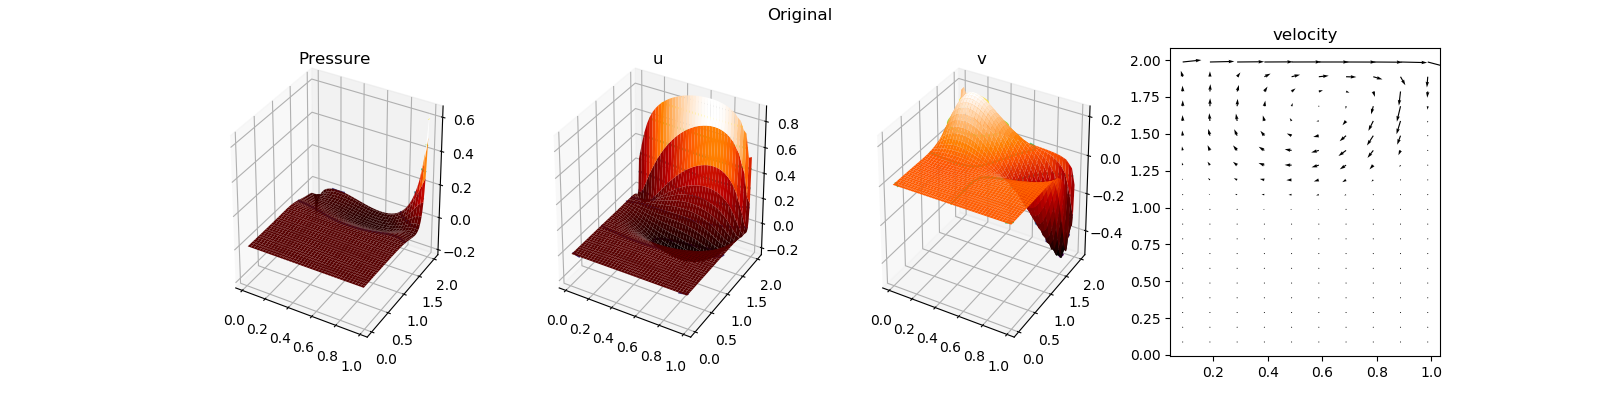
\includegraphics[width=1.35\textwidth]{vortices/original.png}

  \hspace{-30mm}
  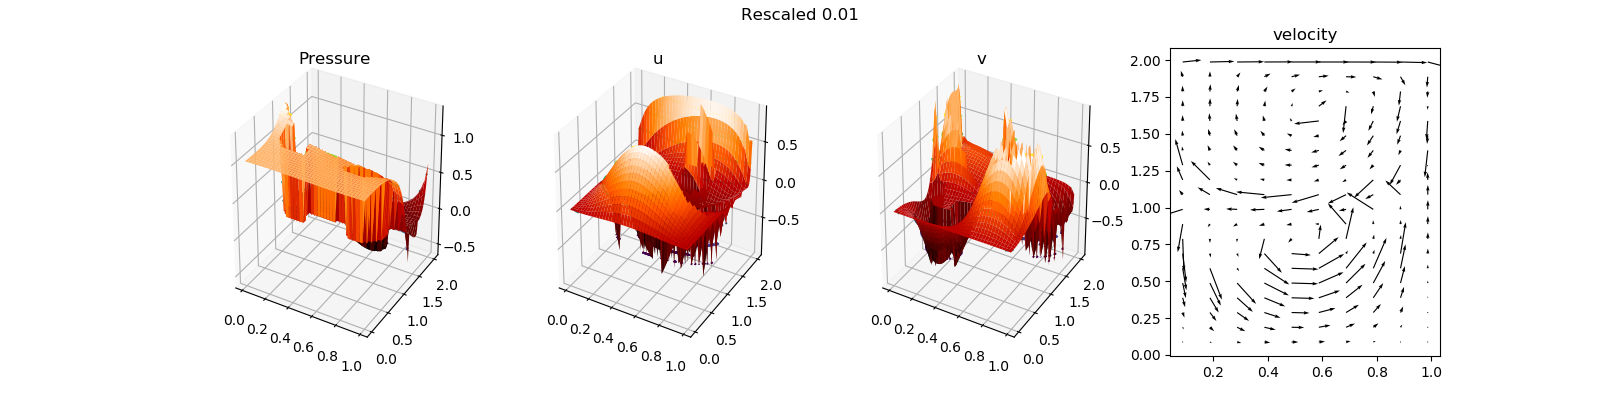
\includegraphics[width=1.35\textwidth]{vortices/rescaled_0_01.png}

  \hspace{-30mm}
  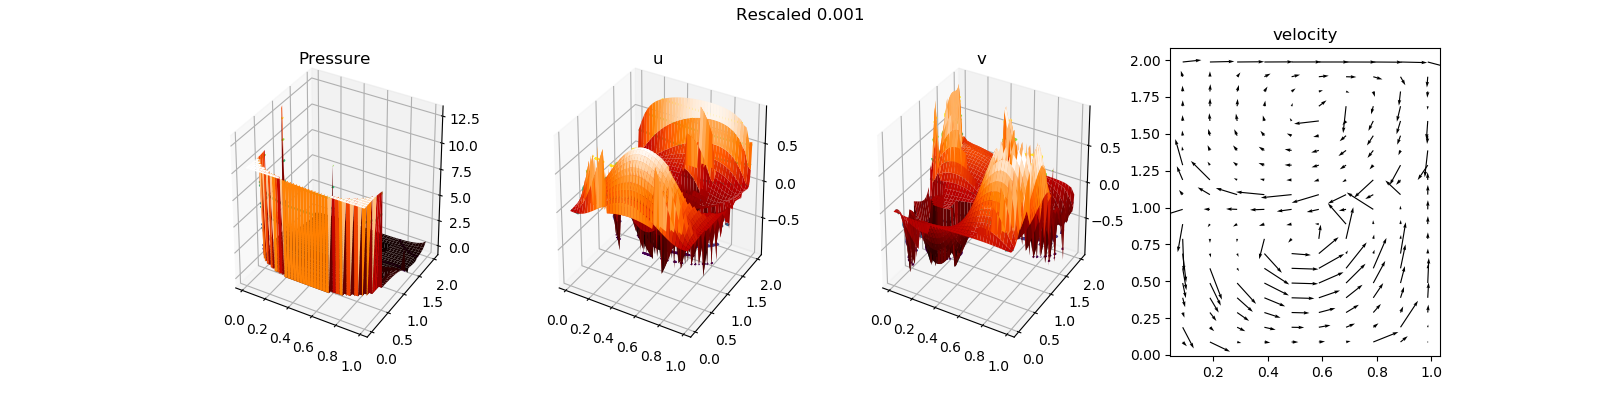
\includegraphics[width=1.35\textwidth]{vortices/rescaled_0_001.png}
  \label{vortex_2}
  \caption{{\bf From left to right, top to bottom:} The computed solutions of $P$, $u$, and $v$.
    The velocity of the solution. Two filtered and rescaled versions of the plot,
    showing an additional vortex beneath the first one, and no additional ones.
    This was run with a 40x80 mesh, over-relaxation of 1.25, beta of 0.75,
    and diffusion coefficient of 32.0}
  }
\end{figure}

Repeating the same method used previously, the center of the vortices ordered by decreasing strength,
appear to be at $(0.5966, 1.651)$, and $(0.5071, 0.7779)$, with strengths $0.969$ and $0.0742$.

The study was again performed with a box with its height four times its width,
the results of which are shown in Figure \ref{vortex_3}.
This should have more vortices, some will harder to resolve than before due to dissipation.
After applying the same method, I found 3 vortices, ordered by decreasing strength,
at $(0.5966, 3.651), (0.5057, 2.775), (0.5278, 1.367)$, with strengths $0.969$, $0.0714$, and $0.000196$.

\begin{figure}[ht]
  \hspace{-30mm}
  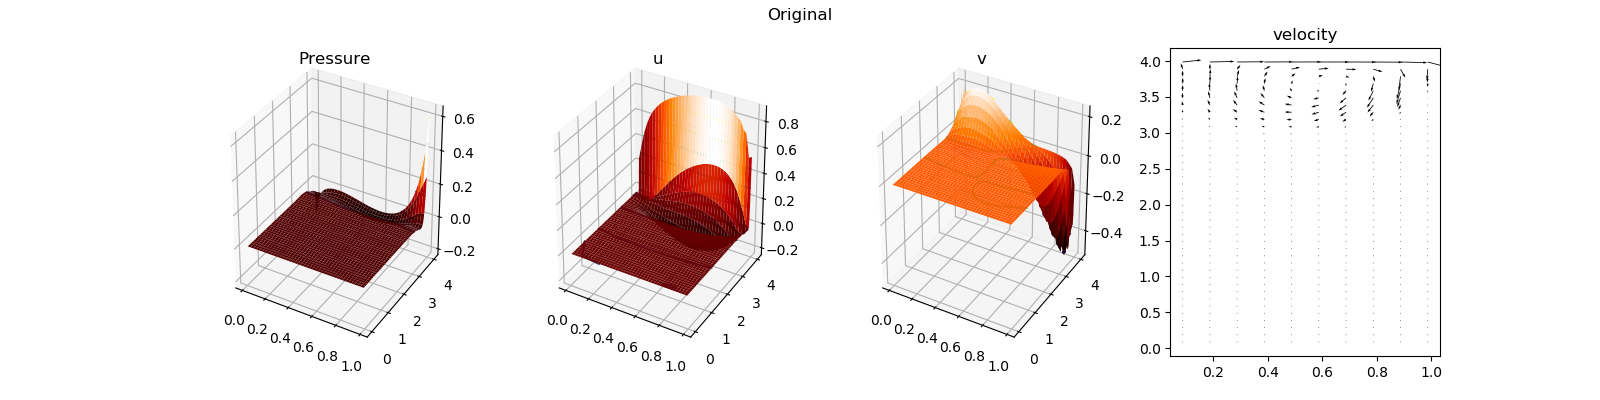
\includegraphics[width=1.35\textwidth]{vortices/original_40x160.png}

  \hspace{-30mm}
  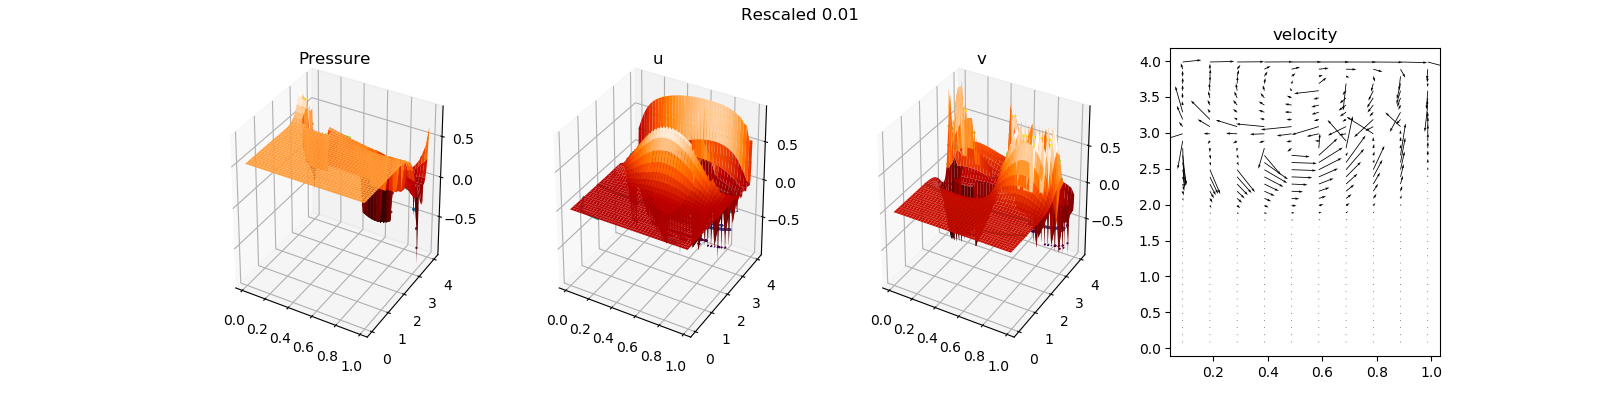
\includegraphics[width=1.35\textwidth]{vortices/rescaled_0_01_40x160.png}

  \hspace{-30mm}
  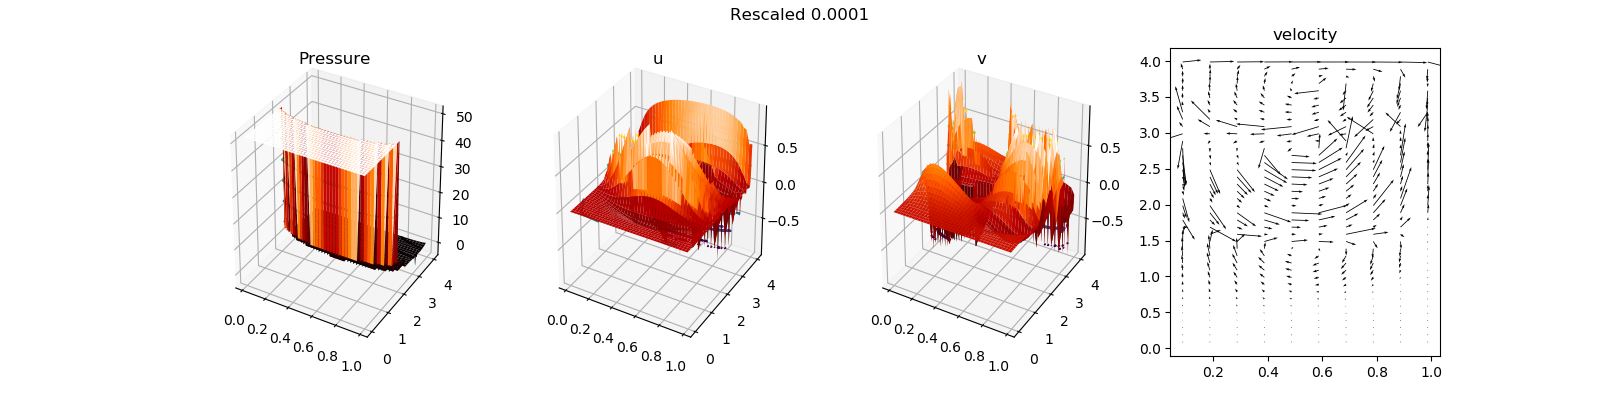
\includegraphics[width=1.35\textwidth]{vortices/rescaled_0_0001_40x160.png}
  \label{vortex_3}
  \caption{{\bf From left to right, top to bottom:} The computed solutions of $P$, $u$, and $v$.
    The velocity of the solution. Two filtered and rescaled versions of the plot,
    showing an additional vortex beneath the first one, and no additional ones.
    This was run with a 40x160 mesh, over-relaxation of 1.25, beta of 0.75,
    and diffusion coefficient of 32.0}
  }
\end{figure}
\end{section}

\end{document}
